\documentclass[11pt,fleqn, oneside,openany]{extbook} % Default font size and left-justified equations

% use this list: https://www.educative.io/blog/google-coding-interview

%%%%%%%%%%%%%%%%%%%%%%%%%%%%%%%%%%%%%%%%%%%%
%               Structure
%%%%%%%%%%%%%%%%%%%%%%%%%%%%%%%%%%%%%%%%%%%%
%%%%%%%%%%%%%%%%%%%%%%%%%%%%%%%%%%%%%%%%%
% The Legrand Orange Book
% Structural Definitions File
% Version 2.0 (9/2/15)
%
% Original author:
% Mathias Legrand (legrand.mathias@gmail.com) with modifications by:
% Vel (vel@latextemplates.com)
% 
% This file has been downloaded from:
% http://www.LaTeXTemplates.com
%
% License:
% CC BY-NC-SA 3.0 (http://creativecommons.org/licenses/by-nc-sa/3.0/)
%
%%%%%%%%%%%%%%%%%%%%%%%%%%%%%%%%%%%%%%%%%

%----------------------------------------------------------------------------------------
%	VARIOUS REQUIRED PACKAGES AND CONFIGURATIONS
%----------------------------------------------------------------------------------------

\usepackage[top=3cm,bottom=3cm,left=3cm,right=3cm,headsep=10pt,a4paper]{geometry} % Page margins

\usepackage{graphicx} % Required for including pictures
\graphicspath{{images/}} % Specifies the directory where pictures are stored

\usepackage{lipsum} % Inserts dummy text

\usepackage{tikz} % Required for drawing custom shapes

\usepackage[english]{babel} % English language/hyphenation

\usepackage{enumitem} % Customize lists
\setlist{nolistsep} % Reduce spacing between bullet points and numbered lists

\usepackage{booktabs} % Required for nicer horizontal rules in tables

\usepackage{xcolor} % Required for specifying colors by name
\definecolor{ocre}{RGB}{243,102,25} % Define the orange color used for highlighting throughout the book

%----------------------------------------------------------------------------------------
%	FONTS
%----------------------------------------------------------------------------------------

\usepackage{avant} % Use the Avantgarde font for headings
%\usepackage{times} % Use the Times font for headings
\usepackage{mathptmx} % Use the Adobe Times Roman as the default text font together with math symbols from the Sym­bol, Chancery and Com­puter Modern fonts

\usepackage{microtype} % Slightly tweak font spacing for aesthetics
\usepackage[utf8]{inputenc} % Required for including letters with accents
\usepackage[T1]{fontenc} % Use 8-bit encoding that has 256 glyphs

%----------------------------------------------------------------------------------------
%	BIBLIOGRAPHY AND INDEX
%----------------------------------------------------------------------------------------

\usepackage[citestyle=numeric,sorting=nyt,sortcites=true,autopunct=true,babel=hyphen,hyperref=true,abbreviate=false,backref=true,backend=biber]{biblatex}
\addbibresource{sources/bibliography.bib}
\defbibheading{bibempty}{}

\usepackage{calc} % For simpler calculation - used for spacing the index letter headings correctly
\usepackage{makeidx} % Required to make an index
\makeindex % Tells LaTeX to create the files required for indexing

%----------------------------------------------------------------------------------------
%	MAIN TABLE OF CONTENTS
%----------------------------------------------------------------------------------------

\usepackage{titletoc} % Required for manipulating the table of contents

\contentsmargin{0cm} % Removes the default margin

% Part text styling
\titlecontents{part}[0cm]
{\addvspace{20pt}\centering\large\bfseries}
{}
{}
{}

% Chapter text styling
\titlecontents{chapter}[1.25cm] % Indentation
{\addvspace{12pt}\large\sffamily\bfseries} % Spacing and font options for chapters
{\color{ocre!60}\contentslabel[\Large\thecontentslabel]{1.25cm}\color{ocre}} % Chapter number
{\color{ocre}}  
{\color{ocre!60}\normalsize\;\titlerule*[.5pc]{.}\;\thecontentspage} % Page number

% Section text styling
\titlecontents{section}[1.25cm] % Indentation
{\addvspace{3pt}\sffamily\bfseries} % Spacing and font options for sections
{\contentslabel[\thecontentslabel]{1.25cm}} % Section number
{}
{\hfill\color{black}\thecontentspage} % Page number
[]

% Subsection text styling
\titlecontents{subsection}[1.25cm] % Indentation
{\addvspace{1pt}\sffamily\small} % Spacing and font options for subsections
{\contentslabel[\thecontentslabel]{1.25cm}} % Subsection number
{}
{\ \titlerule*[.5pc]{.}\;\thecontentspage} % Page number
[]

% List of figures
\titlecontents{figure}[0em]
{\addvspace{-5pt}\sffamily}
{\thecontentslabel\hspace*{1em}}
{}
{\ \titlerule*[.5pc]{.}\;\thecontentspage}
[]

% List of tables
\titlecontents{table}[0em]
{\addvspace{-5pt}\sffamily}
{\thecontentslabel\hspace*{1em}}
{}
{\ \titlerule*[.5pc]{.}\;\thecontentspage}
[]

%----------------------------------------------------------------------------------------
%	MINI TABLE OF CONTENTS IN PART HEADS
%----------------------------------------------------------------------------------------

% Chapter text styling
\titlecontents{lchapter}[0em] % Indenting
{\addvspace{15pt}\large\sffamily\bfseries} % Spacing and font options for chapters
{\color{ocre}\contentslabel[\Large\thecontentslabel]{1.25cm}\color{ocre}} % Chapter number
{}  
{\color{ocre}\normalsize\sffamily\bfseries\;\titlerule*[.5pc]{.}\;\thecontentspage} % Page number

% Section text styling
\titlecontents{lsection}[0em] % Indenting
{\sffamily\small} % Spacing and font options for sections
{\contentslabel[\thecontentslabel]{1.25cm}} % Section number
{}
{}

% Subsection text styling
\titlecontents{lsubsection}[.5em] % Indentation
{\normalfont\footnotesize\sffamily} % Font settings
{}
{}
{}

%----------------------------------------------------------------------------------------
%	PAGE HEADERS
%----------------------------------------------------------------------------------------

\usepackage{fancyhdr} % Required for header and footer configuration

\pagestyle{fancy}
\renewcommand{\chaptermark}[1]{\markboth{\sffamily\normalsize\bfseries\chaptername\ \thechapter.\ #1}{}} % Chapter text font settings
\renewcommand{\sectionmark}[1]{\markright{\sffamily\normalsize\thesection\hspace{5pt}#1}{}} % Section text font settings
\fancyhf{} \fancyhead[LE,RO]{\sffamily\normalsize\thepage} % Font setting for the page number in the header
\fancyhead[LO]{\rightmark} % Print the nearest section name on the left side of odd pages
\fancyhead[RE]{\leftmark} % Print the current chapter name on the right side of even pages
\renewcommand{\headrulewidth}{0.5pt} % Width of the rule under the header
\addtolength{\headheight}{2.5pt} % Increase the spacing around the header slightly
\renewcommand{\footrulewidth}{0pt} % Removes the rule in the footer
\fancypagestyle{plain}{\fancyhead{}\renewcommand{\headrulewidth}{0pt}} % Style for when a plain pagestyle is specified

% Removes the header from odd empty pages at the end of chapters
\makeatletter
\renewcommand{\cleardoublepage}{
\clearpage\ifodd\c@page\else
\hbox{}
\vspace*{\fill}
\thispagestyle{empty}
\newpage
\fi}

%----------------------------------------------------------------------------------------
%	THEOREM STYLES
%----------------------------------------------------------------------------------------


\usepackage{amsmath,amsfonts,amssymb,amsthm,mathtools} % For math equations, theorems, symbols, etc
\DeclarePairedDelimiter\ceil{\lceil}{\rceil}
\DeclarePairedDelimiter\floor{\lfloor}{\rfloor}

\newcommand{\intoo}[2]{\mathopen{]}#1\,;#2\mathclose{[}}
\newcommand{\ud}{\mathop{\mathrm{{}d}}\mathopen{}}
\newcommand{\intff}[2]{\mathopen{[}#1\,;#2\mathclose{]}}
\newtheorem{notation}{Notation}[chapter]

% Boxed/framed environments
\newtheoremstyle{ocrenumbox}% % Theorem style name
{0pt}% Space above
{0pt}% Space below
{\normalfont}% % Body font
{}% Indent amount
{\small\bf\sffamily\color{ocre}}% % Theorem head font
{\;}% Punctuation after theorem head
{0.25em}% Space after theorem head
{\small\sffamily\color{ocre}\thmname{#1}\nobreakspace\thmnumber{\@ifnotempty{#1}{}\@upn{#2}}% Theorem text (e.g. Theorem 2.1)
\thmnote{\nobreakspace\the\thm@notefont\sffamily\bfseries\color{black}---\nobreakspace#3.}} % Optional theorem note
\renewcommand{\qedsymbol}{$\blacksquare$}% Optional qed square

\newtheoremstyle{blacknumex}% Theorem style name
{5pt}% Space above
{5pt}% Space below
{\normalfont}% Body font
{} % Indent amount
{\small\bf\sffamily}% Theorem head font
{\;}% Punctuation after theorem head
{0.25em}% Space after theorem head
{\small\sffamily{\tiny\ensuremath{\blacksquare}}\nobreakspace\thmname{#1}\nobreakspace\thmnumber{\@ifnotempty{#1}{}\@upn{#2}}% Theorem text (e.g. Theorem 2.1)
\thmnote{\nobreakspace\the\thm@notefont\sffamily\bfseries---\nobreakspace#3.}}% Optional theorem note

\newtheoremstyle{blacknumbox} % Theorem style name
{0pt}% Space above
{0pt}% Space below
{\normalfont}% Body font
{}% Indent amount
{\small\bf\sffamily}% Theorem head font
{\;}% Punctuation after theorem head
{0.25em}% Space after theorem head
{\small\sffamily\thmname{#1}\nobreakspace\thmnumber{\@ifnotempty{#1}{}\@upn{#2}}% Theorem text (e.g. Theorem 2.1)
\thmnote{\nobreakspace\the\thm@notefont\sffamily\bfseries---\nobreakspace#3.}}% Optional theorem note

% Non-boxed/non-framed environments
\newtheoremstyle{ocrenum}% % Theorem style name
{5pt}% Space above
{5pt}% Space below
{\normalfont}% % Body font
{}% Indent amount
{\small\bf\sffamily\color{ocre}}% % Theorem head font
{\;}% Punctuation after theorem head
{0.25em}% Space after theorem head
{\small\sffamily\color{ocre}\thmname{#1}\nobreakspace\thmnumber{\@ifnotempty{#1}{}\@upn{#2}}% Theorem text (e.g. Theorem 2.1)
\thmnote{\nobreakspace\the\thm@notefont\sffamily\bfseries\color{black}---\nobreakspace#3.}} % Optional theorem note
\renewcommand{\qedsymbol}{$\blacksquare$}% Optional qed square
\makeatother

% Defines the theorem text style for each type of theorem to one of the three styles above
\newcounter{dummy} 
\numberwithin{dummy}{section}
\theoremstyle{ocrenumbox}
\newtheorem{theoremeT}[dummy]{Theorem}

\newtheorem{problem}{Exercise}[chapter]
\newtheorem{exerciseT}{Problem}
\theoremstyle{blacknumex}
\newtheorem{solution}{Solution}[chapter]
\newtheorem{solutionT}{solution}[chapter]
\theoremstyle{blacknumex}
\newtheorem{exampleT}{Example}[chapter]
\theoremstyle{blacknumbox}
\newtheorem{vocabulary}{Vocabulary}[chapter]
\newtheorem{definitionT}{Definition}[section]
\newtheorem{corollaryT}[dummy]{Corollary}
\theoremstyle{ocrenum}
\newtheorem{proposition}[dummy]{Proposition}

%----------------------------------------------------------------------------------------
%	DEFINITION OF COLORED BOXES
%----------------------------------------------------------------------------------------

\RequirePackage[framemethod=default]{mdframed} % Required for creating the theorem, definition, exercise and corollary boxes

% Theorem box
\newmdenv[skipabove=7pt,
skipbelow=7pt,
backgroundcolor=black!5,
linecolor=ocre,
innerleftmargin=5pt,
innerrightmargin=5pt,
innertopmargin=5pt,
leftmargin=0cm,
rightmargin=0cm,
innerbottommargin=5pt]{tBox}

% Exercise box	  
\newmdenv[skipabove=7pt,
skipbelow=7pt,
rightline=false,
leftline=true,
topline=false,
bottomline=false,
backgroundcolor=ocre!10,
linecolor=ocre,
innerleftmargin=5pt,
innerrightmargin=5pt,
innertopmargin=5pt,
innerbottommargin=5pt,
leftmargin=0cm,
rightmargin=0cm,
linewidth=4pt]{eBox}	

% Definition box
\newmdenv[skipabove=7pt,
skipbelow=7pt,
rightline=false,
leftline=true,
topline=false,
bottomline=false,
linecolor=ocre,
innerleftmargin=5pt,
innerrightmargin=5pt,
innertopmargin=0pt,
leftmargin=0cm,
rightmargin=0cm,
linewidth=4pt,
innerbottommargin=0pt]{dBox}	

% Corollary box
\newmdenv[skipabove=7pt,
skipbelow=7pt,
rightline=false,
leftline=true,
topline=false,
bottomline=false,
linecolor=gray,
backgroundcolor=black!5,
innerleftmargin=5pt,
innerrightmargin=5pt,
innertopmargin=5pt,
leftmargin=0cm,
rightmargin=0cm,
linewidth=4pt,
innerbottommargin=5pt]{cBox}

% Creates an environment for each type of theorem and assigns it a theorem text style from the "Theorem Styles" section above and a colored box from above
\newenvironment{theorem}{\begin{tBox}\begin{theoremeT}}{\end{theoremeT}\end{tBox}}
\newenvironment{exercise}{\begin{eBox}\begin{exerciseT}}{\hfill{\color{ocre}\tiny\ensuremath{\blacksquare}}\end{exerciseT}\end{eBox}}				  
\newenvironment{definition}{\begin{dBox}\begin{definitionT}}{\end{definitionT}\end{dBox}}	
\newenvironment{example}{\begin{exampleT}}{\hfill{\tiny\ensuremath{\blacksquare}}\end{exampleT}}		
\newenvironment{corollary}{\begin{cBox}\begin{corollaryT}}{\end{corollaryT}\end{cBox}}	

%----------------------------------------------------------------------------------------
%	REMARK ENVIRONMENT
%----------------------------------------------------------------------------------------

\newenvironment{remark}{\par\vspace{10pt}\small % Vertical white space above the remark and smaller font size
\begin{list}{}{
\leftmargin=35pt % Indentation on the left
\rightmargin=25pt}\item\ignorespaces % Indentation on the right
\makebox[-2.5pt]{\begin{tikzpicture}[overlay]
\node[draw=ocre!60,line width=1pt,circle,fill=ocre!25,font=\sffamily\bfseries,inner sep=2pt,outer sep=0pt] at (-15pt,0pt){\textcolor{ocre}{R}};\end{tikzpicture}} % Orange R in a circle
\advance\baselineskip -1pt}{\end{list}\vskip5pt} % Tighter line spacing and white space after remark

%----------------------------------------------------------------------------------------
%	SECTION NUMBERING IN THE MARGIN
%----------------------------------------------------------------------------------------

\makeatletter
\renewcommand{\@seccntformat}[1]{\llap{\textcolor{ocre}{\csname the#1\endcsname}\hspace{1em}}}                    
\renewcommand{\section}{\@startsection{section}{1}{\z@}
{-4ex \@plus -1ex \@minus -.4ex}
{1ex \@plus.2ex }
{\normalfont\large\sffamily\bfseries}}
\renewcommand{\subsection}{\@startsection {subsection}{2}{\z@}
{-3ex \@plus -0.1ex \@minus -.4ex}
{0.5ex \@plus.2ex }
{\normalfont\sffamily\bfseries}}
\renewcommand{\subsubsection}{\@startsection {subsubsection}{3}{\z@}
{-2ex \@plus -0.1ex \@minus -.2ex}
{.2ex \@plus.2ex }
{\normalfont\small\sffamily\bfseries}}                        
\renewcommand\paragraph{\@startsection{paragraph}{4}{\z@}
{-2ex \@plus-.2ex \@minus .2ex}
{.1ex}
{\normalfont\small\sffamily\bfseries}}

%----------------------------------------------------------------------------------------
%	PART HEADINGS
%----------------------------------------------------------------------------------------

% numbered part in the table of contents
\newcommand{\@mypartnumtocformat}[2]{%
\setlength\fboxsep{0pt}%
\noindent\colorbox{ocre!20}{\strut\parbox[c][.7cm]{\ecart}{\color{ocre!70}\Large\sffamily\bfseries\centering#1}}\hskip\esp\colorbox{ocre!40}{\strut\parbox[c][.7cm]{\linewidth-\ecart-\esp}{\Large\sffamily\centering#2}}}%
%%%%%%%%%%%%%%%%%%%%%%%%%%%%%%%%%%
% unnumbered part in the table of contents
\newcommand{\@myparttocformat}[1]{%
\setlength\fboxsep{0pt}%
\noindent\colorbox{ocre!40}{\strut\parbox[c][.7cm]{\linewidth}{\Large\sffamily\centering#1}}}%
%%%%%%%%%%%%%%%%%%%%%%%%%%%%%%%%%%
\newlength\esp
\setlength\esp{4pt}
\newlength\ecart
\setlength\ecart{1.2cm-\esp}
\newcommand{\thepartimage}{}%
\newcommand{\partimage}[1]{\renewcommand{\thepartimage}{#1}}%
\def\@part[#1]#2{%
\ifnum \c@secnumdepth >-2\relax%
\refstepcounter{part}%
\addcontentsline{toc}{part}{\texorpdfstring{\protect\@mypartnumtocformat{\thepart}{#1}}{\partname~\thepart\ ---\ #1}}
\else%
\addcontentsline{toc}{part}{\texorpdfstring{\protect\@myparttocformat{#1}}{#1}}%
\fi%
\startcontents%
\markboth{}{}%
{\thispagestyle{empty}%
\begin{tikzpicture}[remember picture,overlay]%
\node at (current page.north west){\begin{tikzpicture}[remember picture,overlay]%	
\fill[ocre!20](0cm,0cm) rectangle (\paperwidth,-\paperheight);
\node[anchor=north] at (4cm,-3.25cm){\color{ocre!40}\fontsize{220}{100}\sffamily\bfseries\@Roman\c@part}; 
\node[anchor=south east] at (\paperwidth-1cm,-\paperheight+1cm){\parbox[t][][t]{8.5cm}{
\printcontents{l}{0}{\setcounter{tocdepth}{1}}%
}};
\node[anchor=north east] at (\paperwidth-1.5cm,-3.25cm){\parbox[t][][t]{15cm}{\strut\raggedleft\color{white}\fontsize{30}{30}\sffamily\bfseries#2}};
\end{tikzpicture}};
\end{tikzpicture}}%
\@endpart}
\def\@spart#1{%
\startcontents%
\phantomsection
{\thispagestyle{empty}%
\begin{tikzpicture}[remember picture,overlay]%
\node at (current page.north west){\begin{tikzpicture}[remember picture,overlay]%	
\fill[ocre!20](0cm,0cm) rectangle (\paperwidth,-\paperheight);
\node[anchor=north east] at (\paperwidth-1.5cm,-3.25cm){\parbox[t][][t]{15cm}{\strut\raggedleft\color{white}\fontsize{30}{30}\sffamily\bfseries#1}};
\end{tikzpicture}};
\end{tikzpicture}}
\addcontentsline{toc}{part}{\texorpdfstring{%
\setlength\fboxsep{0pt}%
\noindent\protect\colorbox{ocre!40}{\strut\protect\parbox[c][.7cm]{\linewidth}{\Large\sffamily\protect\centering #1\quad\mbox{}}}}{#1}}%
\@endpart}
\def\@endpart{\vfil\newpage
\if@twoside
\if@openright
\null
\thispagestyle{empty}%
\newpage
\fi
\fi
\if@tempswa
\twocolumn
\fi}

%----------------------------------------------------------------------------------------
%	CHAPTER HEADINGS
%----------------------------------------------------------------------------------------

% A switch to conditionally include a picture, implemented by  Christian Hupfer
\newif\ifusechapterimage
\usechapterimagetrue
\newcommand{\thechapterimage}{}%
\newcommand{\chapterimage}[1]{\ifusechapterimage\renewcommand{\thechapterimage}{#1}\fi}%
\def\@makechapterhead#1{%
{\parindent \z@ \raggedright \normalfont
\ifnum \c@secnumdepth >\m@ne
\if@mainmatter
\begin{tikzpicture}[remember picture,overlay]
\node at (current page.north west)
{\begin{tikzpicture}[remember picture,overlay]
\node[anchor=north west,inner sep=0pt] at (0,0) {\ifusechapterimage\includegraphics[width=\paperwidth]{\thechapterimage}\fi};
\draw[anchor=west] (\Gm@lmargin,-4cm) node [line width=2pt,rounded corners=15pt,draw=ocre,fill=white,fill opacity=0.5,inner sep=15pt]{\strut\makebox[22cm]{}};
\draw[anchor=west] (\Gm@lmargin+.3cm,-4cm) node {\huge\sffamily\bfseries\color{black}\thechapter. #1\strut};
\end{tikzpicture}};
\end{tikzpicture}
\else
\begin{tikzpicture}[remember picture,overlay]
\node at (current page.north west)
{\begin{tikzpicture}[remember picture,overlay]
\node[anchor=north west,inner sep=0pt] at (0,0) {\ifusechapterimage\includegraphics[width=\paperwidth]{\thechapterimage}\fi};
\draw[anchor=west] (\Gm@lmargin,-4cm) node [line width=2pt,rounded corners=15pt,draw=ocre,fill=white,fill opacity=0.5,inner sep=15pt]{\strut\makebox[22cm]{}};
\draw[anchor=west] (\Gm@lmargin+.3cm,-4cm) node {\huge\sffamily\bfseries\color{black}#1\strut};
\end{tikzpicture}};
\end{tikzpicture}
\fi\fi\par\vspace*{100\p@}}}

%-------------------------------------------

\def\@makeschapterhead#1{%
\begin{tikzpicture}[remember picture,overlay]
\node at (current page.north west)
{\begin{tikzpicture}[remember picture,overlay]
\node[anchor=north west,inner sep=0pt] at (0,0) {\ifusechapterimage\includegraphics[width=\paperwidth]{\thechapterimage}\fi};
\draw[anchor=west] (\Gm@lmargin,-4cm) node [line width=2pt,rounded corners=15pt,draw=ocre,fill=white,fill opacity=0.5,inner sep=15pt]{\strut\makebox[22cm]{}};
\draw[anchor=west] (\Gm@lmargin+.3cm,-4cm) node {\huge\sffamily\bfseries\color{black}#1\strut};
\end{tikzpicture}};
\end{tikzpicture}
\par\vspace*{100\p@}}
\makeatother

%----------------------------------------------------------------------------------------
%	HYPERLINKS IN THE DOCUMENTS
%----------------------------------------------------------------------------------------

\usepackage{hyperref}
\hypersetup{hidelinks,backref=true,pagebackref=true,hyperindex=true,colorlinks=false,breaklinks=true,urlcolor= ocre,bookmarks=true,bookmarksopen=false,pdftitle={Title},pdfauthor={Author}}
\usepackage{bookmark}
\bookmarksetup{
open,
numbered,
addtohook={%
\ifnum\bookmarkget{level}=0 % chapter
\bookmarksetup{bold}%
\fi
\ifnum\bookmarkget{level}=-1 % part
\bookmarksetup{color=ocre,bold}%
\fi
}
}

%----------------------------------------------------------------------------------------
%	LISTINGS
%----------------------------------------------------------------------------------------
%----------------------------------------------------------------------------------------
%	LISTINGS
%----------------------------------------------------------------------------------------
\usepackage{listings}
\lstset{language=C++}
\lstset{
	basicstyle=\footnotesize\ttfamily,
	breaklines=true,
	showstringspaces=false,
	numbers=left,
	backgroundcolor=\color{bgcolor},
	commentstyle=\color{gray},
	keywordstyle=\color{blue},
	keywordstyle=[2]\color{teal},   % cyan or teal can also be a good choice, use \bfseries for bold
	frame=none,                     % adds a frame around the code
	tabsize=2,                      % sets default tabsize to 2 spaces
	captionpos=b,                   % sets the caption-position to bottom
	morekeywords=[2]{}              % if you want to add more keywords to the set
	__
}

\definecolor{mygreen}{RGB}{28,172,0} % color values Red, Green, Blue
\definecolor{mylilas}{RGB}{170,55,241}
\lstset{language=Matlab,%
    %basicstyle=\color{red},
    breaklines=true,%
    morekeywords={matlab2tikz},
    keywordstyle=\color{blue},%
    morekeywords=[2]{1}, keywordstyle=[2]{\color{black}},
    identifierstyle=\color{black},%
    stringstyle=\color{mylilas},
    commentstyle=\color{mygreen},%
    showstringspaces=false,%without this there will be a symbol in the places where there is a space
    numbers=left,%
    numberstyle={\tiny \color{black}},% size of the numbers
    numbersep=9pt, % this defines how far the numbers are from the text
    emph=[1]{for,end,break},emphstyle=[1]\color{red}, %some words to emphasise
    %emph=[2]{word1,word2}, emphstyle=[2]{style},    
}

\usepackage{color}
\definecolor{bgcolor}{rgb}{0.98,0.98,0.98}


%----------------------------------------------------------------------------------------

%	QandA

%----------------------------------------------------------------------------------------

\newenvironment{QandA}{\begin{enumerate}[label=\bfseries Q.\arabic*.,leftmargin=2em,rightmargin=2em]\bfseries}{\end{enumerate}}
\newenvironment{answered}{\par\normalfont}{}
%----------------------------------------------------------------------------------------
%	ALGORITHM
%----------------------------------------------------------------------------------------
\usepackage[]{algorithm2e}

\RestyleAlgo{boxruled}
\usepackage{mdframed,framed}

\SetKwProg{Fn}{Function}{}{}
\SetKwRepeat{Do}{do}{while}%
\SetKwFunction{CreateHashSet}{CreateHashSet<int>}


\DeclarePairedDelimiter\abs{\lvert}{\rvert}%
\DeclarePairedDelimiter\norm{\lVert}{\rVert}%

% Swap the definition of \abs* and \norm*, so that \abs
% and \norm resizes the size of the brackets, and the 
% starred version does not.
\makeatletter
\let\oldabs\abs
\def\abs{\@ifstar{\oldabs}{\oldabs*}}
%
\let\oldnorm\norm
\def\norm{\@ifstar{\oldnorm}{\oldnorm*}}
\makeatother

\usepackage[makeroom]{cancel}


\interfootnotelinepenalty=10000

\begin{document}

%\frontmatter
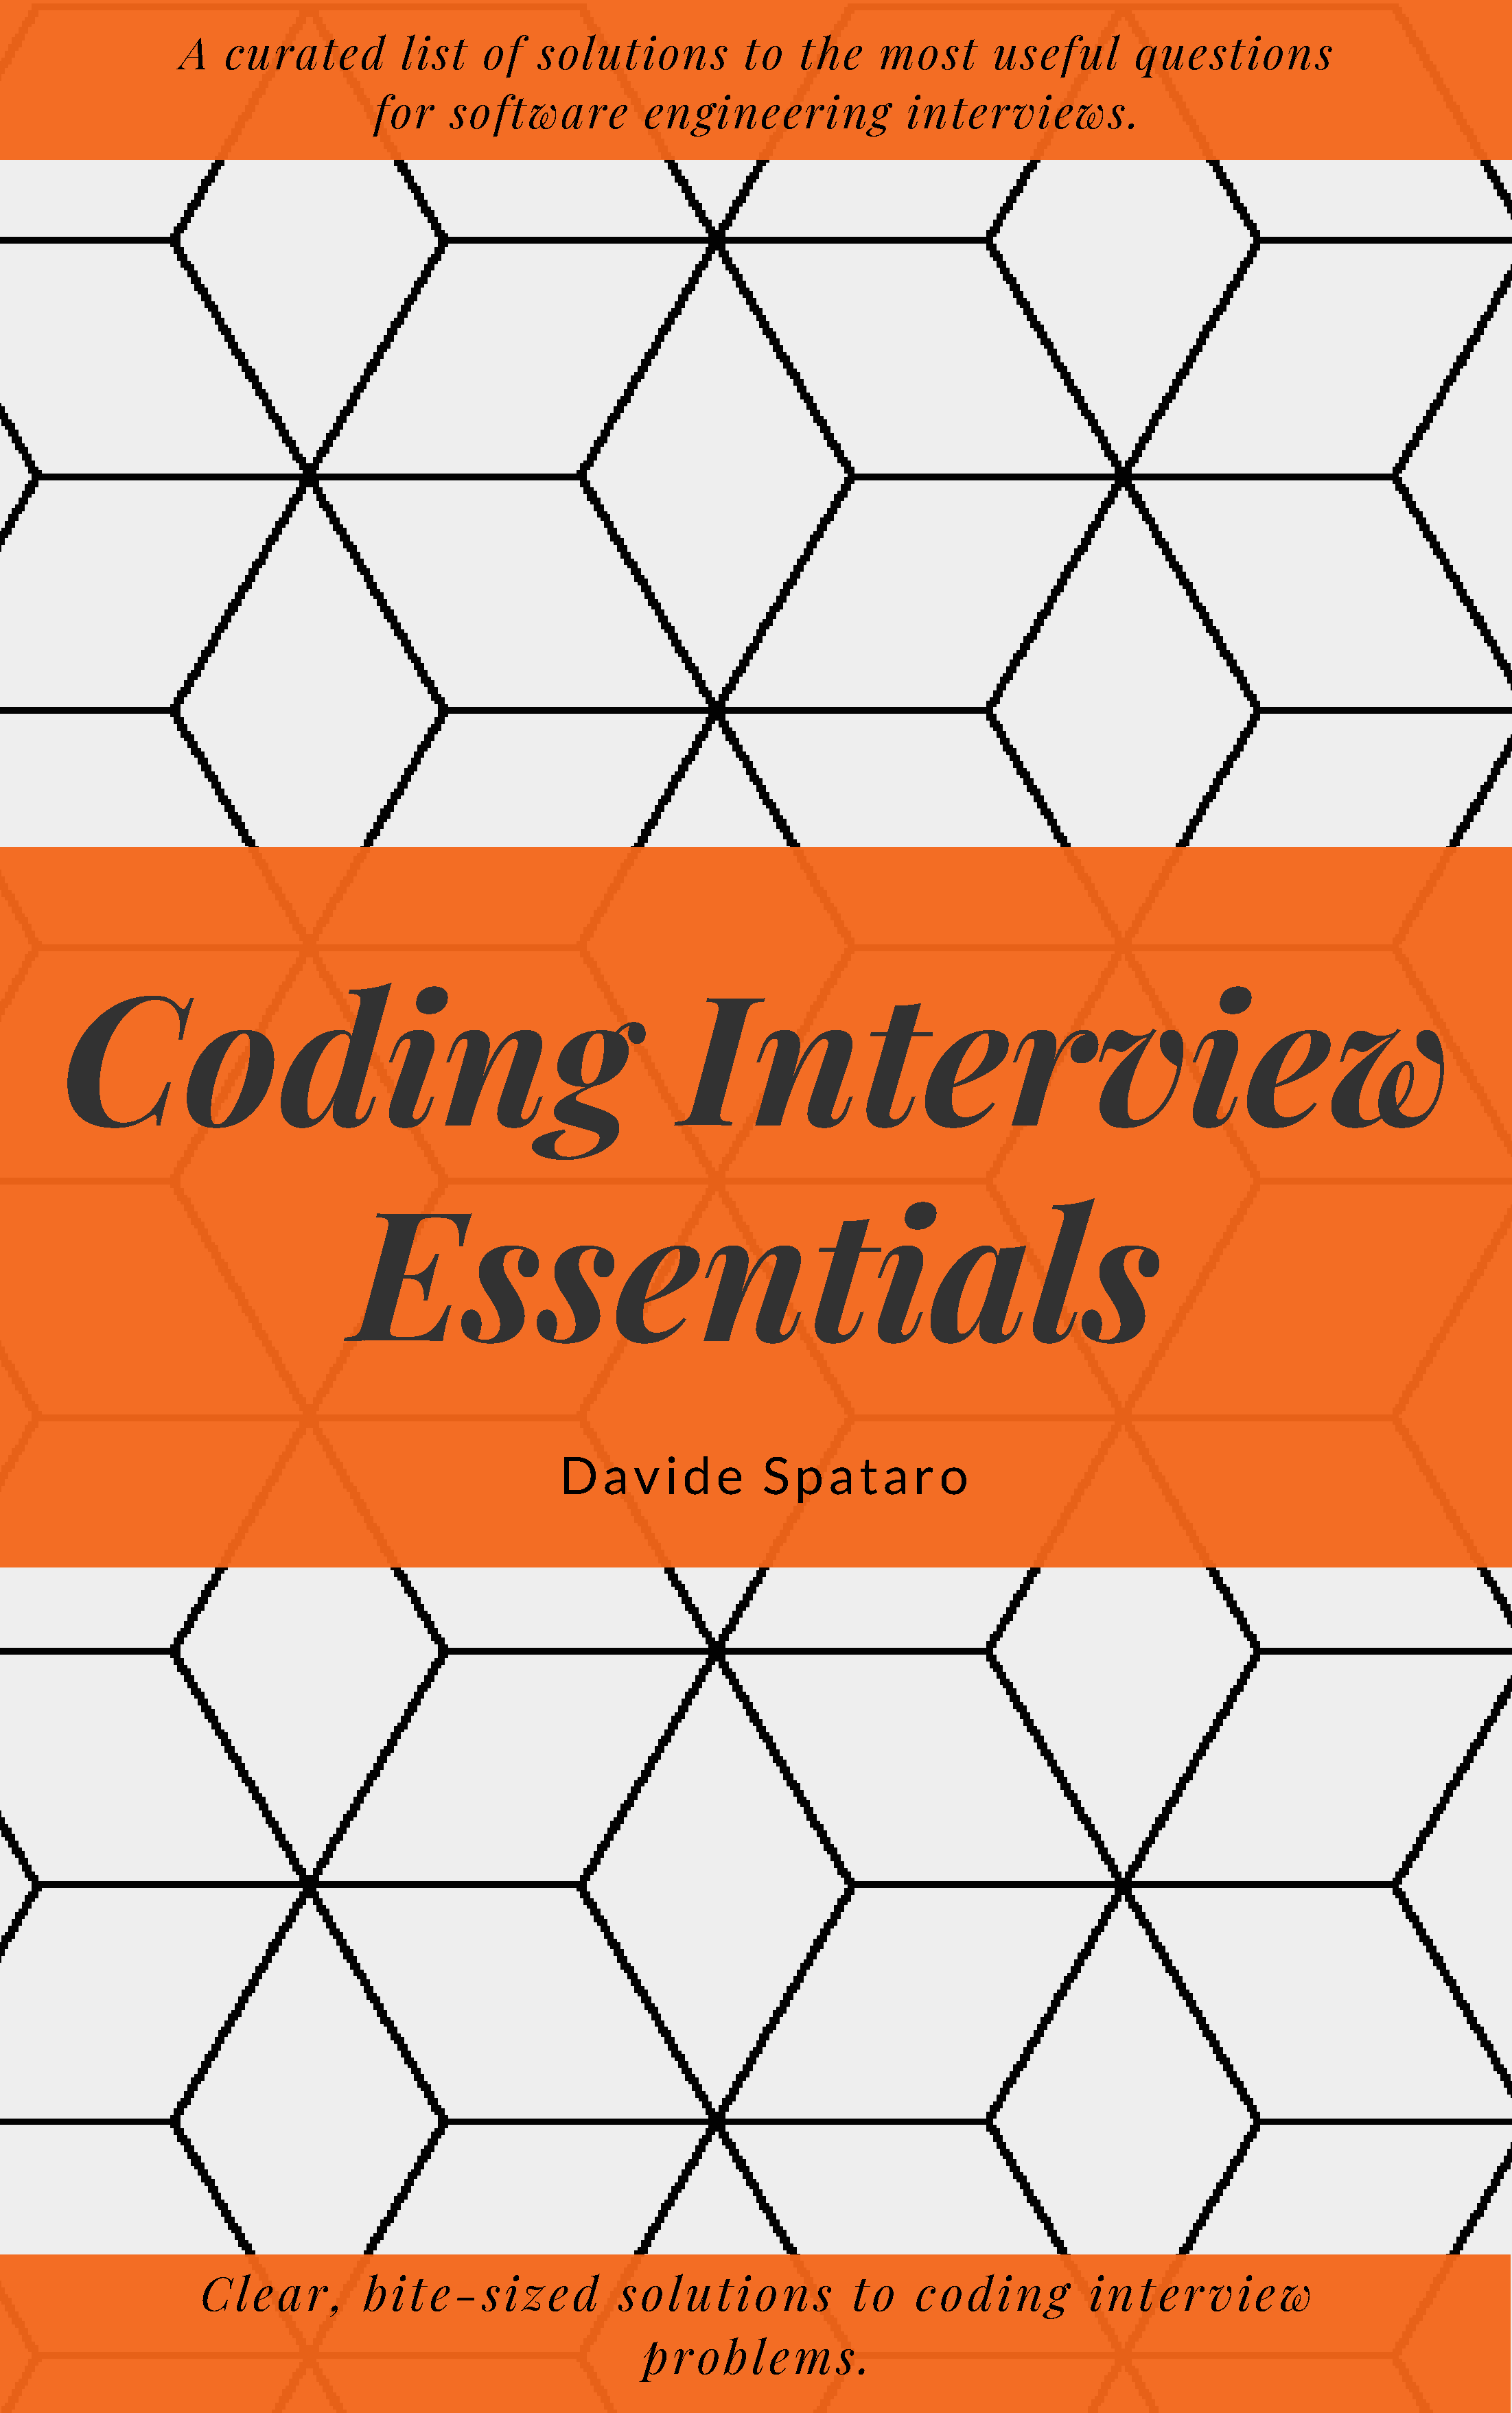
\includepdf[pages=1, fitpaper]{sources/front_cover_image.pdf}
%%\begingroup
%\thispagestyle{empty}
%\begin{tikzpicture}[remember picture,overlay]
%  \coordinate [below=12cm] (midpoint) at (current page.north);
%  \node at (current page.north west)
%  {\begin{tikzpicture}[remember picture,overlay]
%      \node[anchor=north west,inner sep=0pt] at (0,0) {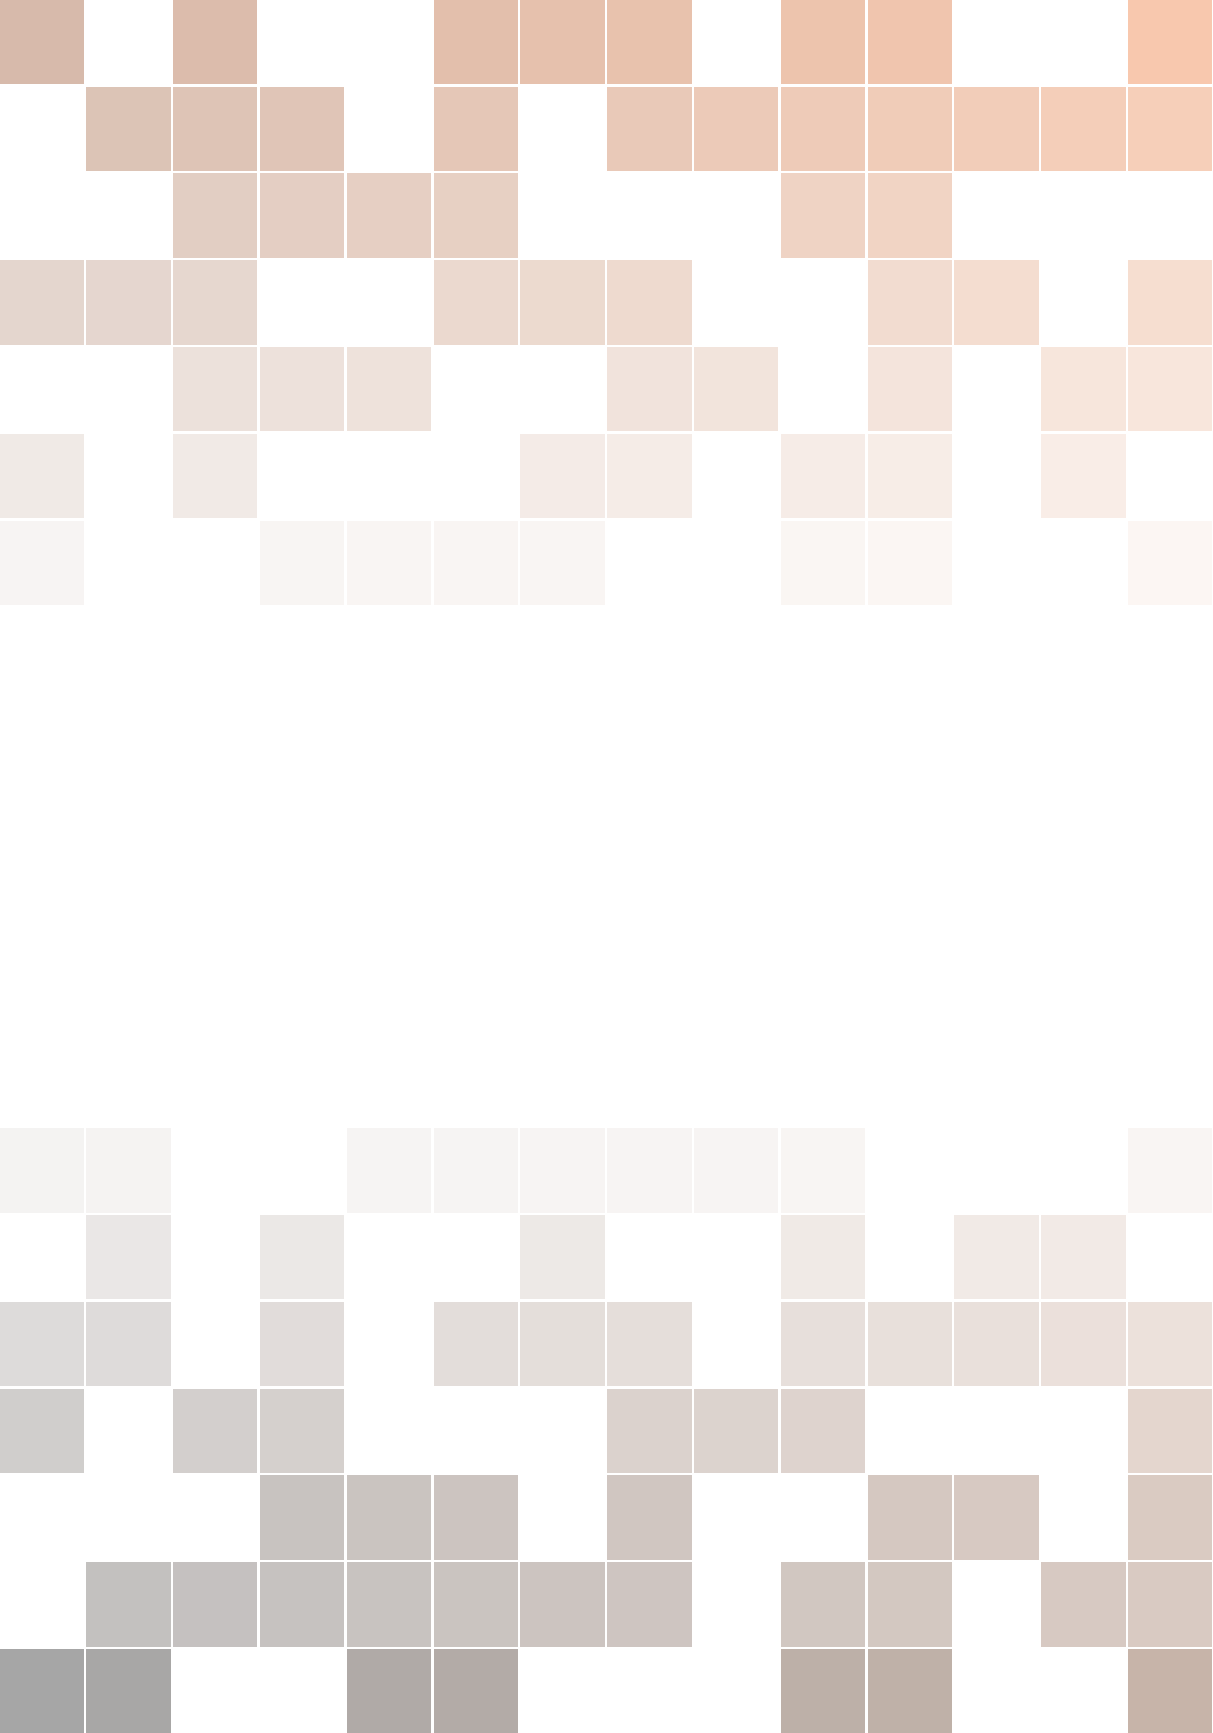
\includegraphics[width=\paperwidth]{images/background}}; % Background image
%\textsl{}
%      \draw[anchor=north] (midpoint) node [fill=ocre!30!white,fill opacity=0.6,text opacity=1,inner sep=1cm]{\Huge\centering\bfseries\sffamily\parbox[c][][t]{\paperwidth}{\centering Coding Interview Essentials\\[15pt] % Book title
%      {\Large - }\\[20pt] % Subtitle
%      {\huge Davide Spataro}}}; % Author name
%    \end{tikzpicture}};
%\end{tikzpicture}
%\vfill
%\endgroup


\includepdf[pages={2},fitpaper=true]{images/book_covers1.pdf}


\usechapterimagefalse % If you don't want to include a chapter image, use this to toggle images off - it can be enabled later with \usechapterimagetrue

%\chapterimage{images/header} % Table of contents heading image

\pagestyle{empty} % No headers

\tableofcontents % Print the table of contents itself

%\lstlistoflistings
%\listoffigures
%\listoftables

\cleardoublepage % Forces the first chapter to start on an odd page so it's on the right

%pagestyle{fancy} % Print headers again

%!TEX root = ../main.tex
%%%%%%%%%%%%%%%%%%%%%%%%%%%%%%%%%%
% Links:
%
% Difficulty:
% Companies: 
%%%%%%%%%%%%%%%%%%%%%%%%%%%%%%%%%%

\chapter{Find the majority element}
\label{ch:majority_element}
\section*{Introduction}
The problem described in this chapter has been asked at Microsoft, Google, Amazon and Yahoo interview for software engineering position and it is considered a problem of easy/medium difficulty.

\section{Problem statement}
\begin{exercise}
Given an array $N$ of size $n$, find the majority element i.e. that element that appears more than $\lfloor \frac{n}{2} \rfloor$ times.
If such element does not exists, returns $-1$.
	\begin{example}
		\hfill \\
		Given the array $[1,2,3,2,2,1,1,1]$, the function returns $1$ because it appears $4$ times in an array of length $8$.
	
	\end{example}

	\begin{example}
		\hfill \\
		Given the input array $[2, 1, 2]$ the function return $2$ because it is greater than $\frac{3}{2}$.
		
	\end{example}

	\begin{example}
		\hfill \\
		Given the input array $[2, 1, 2,3,4,5]$ the function return $-1$no element appear more than $3$ times.
		
	\end{example}

\end{exercise}

\section{Clarification Questions}

\begin{QandA}
	\item What are the minimum and maximum value an element of the array can take? 
	\begin{answered}
		\textit{The minimum and maximum values are $[-10^9, 10^9]$, respectively}.
		This is a good question to ask because if the range is small then we can apply a solution based on bucket counting.
	\end{answered}

	\item Can the input array $N$ be modified or shuffled. 
	\begin{answered}
		\textit{Yes, the input array can be modified.}
	\end{answered}
\end{QandA}

\section{Discussion}
\label{majority_element:sec:discussion}
We will have a look at three different solution for this problem. We will start our discussion by having a look in section \ref{majority_element:sec:bruteforce} at the brute-force approach. Section section \ref{majority_element:sec:sorting} will describe an approach that uses sorting to improve the time complexity on the brute-force approach. Lastly in section \ref{majority_element:sec:linear} we will the optimal approach.

\subsection{Brute-force}
\label{majority_element:sec:bruteforce}
The brute force solution is brutally simple and consist in, looping through the array, and for each element counting how many times it occurs in the input array. This approach, despite its simplicity should not be the one provided to the interviewer, as it is far from the optimum and the interviewer is certainly expecting more from us.
Listing \ref{list:majority_element:bruteforce} shows a possible implementation of this idea. 

\lstinputlisting[language=c++, caption={Sample Caption},label=list:majority_element:bruteforce]{sources/majority_element/majority_element_solution1.cpp}


\subsection{Hash-map approach}
\label{majority_element:sec:hashmap}

The idea described in section \ref{majority_element:sec:bruteforce} can be improved by using an hash-map to store the number of occurrence of each element in the input array. There cannot be more than $n$ different numbers in the the array $N$, thus with a single pass of the input and with a linear cost in space we can calculate the number of occurrence of each element and check if any of the counters at any points gets higher than $\lfloor \frac{n}{2} \rfloor$.

A possible implementation of this approach is shown in Listing \ref{list:majority_element:hashmap}.
The complexity of this approach is $O(n)$ for both space and time. In-fact, in the worst case all the element of the input array are only read and stored once.

\lstinputlisting[language=c++, caption={Solution to the problem of finding the majority element in an array using hash-map.},label=list:majority_element:hashmap]{sources/majority_element/majority_element_solution2.cpp}

\subsection{Sorting - Counting}
\label{majority_element:sec:sorting}
The approach described in section \ref{majority_element:sec:hashmap} is definitely faster then the quadratic brute-force but at a linear price in space. In order not to pay the price in space but to lower the time complexity down from quadratic, we could rely on the fact that in a sort collection of elements all equal elements appear grouped together e.g. in $[1,1,2,2,3,3,3,4,4,9,9]$, all the $1$s appear at the beginning of the array, followed by all the $2$s, etc. We can then count the number of occurrences of each element in constant space as shown in Listing \ref{list:majority_element:sorting}. The complexity of this approach is bounded by the sorting which costs $O(nlog(n)$ time.

\lstinputlisting[language=c++, caption={Solution  to the problem of finding the majority element in an array using sorting.},label=list:majority_element:sorting]{sources/majority_element/majority_element_solution3.cpp}

\subsection{Sorting - Median}
\label{majority_element:sec:median}
There is however, another way of taking advantage of the fact that we have a sorted collection. The key idea here is that if a majority element exists than, this element \textbf{must be the median}. After all, by definition , the median if the element that is right in the middle of the sorted collection. Since the majority element will be occupy \textbf{more} than half positions of the array, it also occupies the median position.
All is necessary after sorting the array, is to check if the median value appear more than $\lfloor \frac{n}{2} \rfloor$ times. 
This idea is implemented in Listing \ref{list:majority_element:median} and has a complexity of $O(nlog(n)$ due to sorting.

\lstinputlisting[language=c++, caption={Linear time constant space solution to the problem of finding the majority element in an array.},label=list:majority_element:median]{sources/majority_element/majority_element_solution4.cpp}

\subsection{Boyer-Moore algorithm}
\label{majority_element:sec:linear}
There is however better way of solving this problem in linear time and constant space i.e. using the Boyer-Moore algorithm\cite{Boyer1991}.

The algorithm uses two variables to maintain an candidate element $el$ of the sequence and its current count $count=0$ (initialized to $0$). It processes the elements one by one and will perform the following operations:
\begin{itemize}
	\item if we are processing the very first element  of the sequence or \inline{count=0}, it will set $count=1$ and $el$ to that element (this is out first candidate).
	\item otherwise, if the element currently processed is equal to \inline{el}it increments the counter i.e. \inline{count = count+1}
	\item if the element currently processed is different, then it decrements the counter i.e. \inline{count = count -1};
\end{itemize}


At the end of this process the variable \inline{el} will contain a candidate majority element. If the array contains a majority element then \inline{el} \textbf{is} the one. The algorithm correctness can be derived from the fact that the counter will be incremented more times than it will be decremented for the majority element. If we cannot assume that a majority element \textbf{always} exists then a second pass  on the array is then necessary, in order to count the number of occurrences of \inline{el} in the input array.

Listing \ref{list:majority_element:moore} shows a possible implementation of the Boyer-Moore algorithm. The complexity of this approach is $O(n)$ time and $O(1)$ space because the input array is scanned twice and only two additional integer variables are used.

\lstinputlisting[language=c++, caption={Linear time constant space solution to the problem of finding the majority element in an array.},label=list:majority_element:moore]{sources/majority_element/majority_element_solution5.cpp}



%!TEX root = ../main.tex
%%%%%%%%%%%%%%%%%%%%%%%%%%%%%%%%%%
% Links:
%
% Difficulty:
% Companies: 
%%%%%%%%%%%%%%%%%%%%%%%%%%%%%%%%%%


%\begin{figure}
%	\centering
%	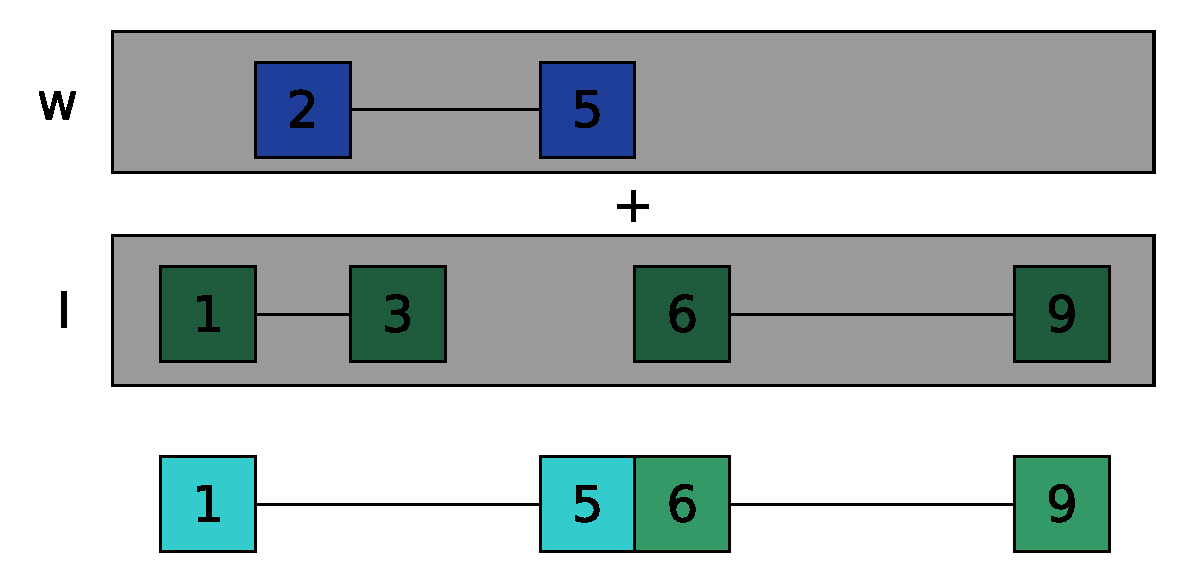
\includegraphics[width=\textwidth]{sources/merge_intervals_2/images/example1}
%	\caption[Sample short cpation]{Sample Caption}.
%	\label{fig:merge_intervals_2:example1}
%\end{figure}

\chapter{Merge Intervals}
\label{ch:merge_intervals_2}
\section*{Introduction}

\section{Problem statement}
\begin{exercise}
\label{example:merge_intervals_2:exercice1}
\begin{verbatim}
	
	Given a sorted list of disjoint (non-overlapping) intervals $I$ and an interval $w$
	insert $w$ into $I$ so that the 
	You may assume that the intervals were initially sorted according to their start times.
	
	Example 1:
	
	Given intervals [1,3],[6,9] insert and merge [2,5] would result in [1,5],[6,9].
	
	Example 2:
	
	Given [1,2],[3,5],[6,7],[8,10],[12,16], insert and merge [4,9] would result in [1,2],[3,10],[12,16].
	
	This is because the new interval [4,9] overlaps with [3,5],[6,7],[8,10].
	
	Make sure the returned intervals are also sorted.
\end{verbatim}

	%example1
	\begin{example}
		\label{example:merge_intervals_2:example1}
		\hfill \\
	
		
	\end{example}

	%example2
	\begin{example}
		\label{example:merge_intervals_2:example2}
		\hfill \\
		
	\end{example}

	\begin{example}
		\hfill \\
	
	\label{ex:merge_intervals_2:example3}
	\end{example}

	\begin{example}
		\hfill \\

	\label{ex:merge_intervals_2:example4}	
	\end{example}
\end{exercise}

\section{Clarification Questions}

\begin{QandA}
	\item 
	\begin{answered}
		\textit{}
	\end{answered}
	
\end{QandA}

\section{Discussion}
\label{merge_intervals_2:sec:discussion}


\subsection{Brute-force}
\label{merge_intervals_2:sec:bruteforce}

\begin{minipage}{\linewidth}
	\lstinputlisting[language=c++, caption={Sample Caption},label=list:merge_intervals_2]{sources/merge_intervals_2/merge_intervals_2_solution1.cpp}
\end{minipage}


\chapter{\CC questionnaire}
   
    \begin{cppquestion}
        \label{cppquestion:q1}
        (Solution \ref{cppquestion:s1} at page \pageref{cppquestion:s1})
        \question \textbf{Which of the following statements is true for the code below:} 
\begin{lstlisting}[language=c++,numbers=none, caption={}]
struct X
{
  A a;
  B b;
  X() : a{}, b{}  {}
};

struct Y : X
{
  C c;
  D d;
  Y() : d{}, c{}  {}
  ~Y() {  }
};                    
\end{lstlisting} 
        \begin{choices}
            \choice Destruction of type \inline{Y} will call member destructors in the following order \inline{A::~A(), B::~B(), D::~D(), C::~C()}
            \choice Destruction of type \inline{Y} will call member destructors in the following order \inline{A::~A(), B::~B(), C::~C(), D::~D()}
            \choice Destruction of type \inline{Y} will call member destructors in the following order \inline{C::~C(), D::~D(), B::~B(), A::~A()}
            \choice Destruction of type \inline{Y} will call member destructors in the following order \inline{D::~D(), C::~C(), B::~B(), A::~A()}
            \choice Destruction of type \inline{Y} will only call destructors of classes \inline{C} and \inline{D} as the destructor of class \inline{X} is not called from \inline{Y::~Y()}
        \end{choices}
\end{cppquestion}
        



\begin{cppquestion}
    \label{cppquestion:q2}
    (Solution \ref{cppquestion:s2} at page \pageref{cppquestion:s2}) 
    \question \textbf{What will be the result of the code below?} 
    \begin{lstlisting}[language=c++,numbers=none, caption={}]
const char* ptr1 = "123456";
const char* ptr2 = "1234567";

if(ptr1 == ptr2)
    printf("same address");
else
    printf("different address");
        \end{lstlisting} 
    \begin{choices}
    \choice \quotes{different address}
    \choice \quotes{same address}
    \choice compilation error
    \choice runtime error
    \end{choices}
\end{cppquestion}


\begin{cppquestion}
    \label{cppquestion:q3}
    (Solution \ref{cppquestion:s3} at page \pageref{cppquestion:s3})
    \question \textbf{Which of the following pointer declarations will allow you to modify the value the pointer points to?} 
    
    \begin{choices}
     \choice \inline{int* ptr;}
     \choice \inline{const int* ptr;}
     \choice \inline{const int* const ptr;}
     \choice \inline{int const* ptr;}
     \choice \inline{int const* const ptr;}
     \choice \inline{int* const ptr;}
    \end{choices}
\end{cppquestion}

\begin{cppquestion}
    \label{cppquestion:q4}
    (Solution \ref{cppquestion:s4} at page \pageref{cppquestion:s4})
    \question \textbf{Which of the following statements are true for the code below?} 
    \begin{lstlisting}[language=c++,numbers=none, caption={}]
class Account
{
  mutable std::mutex m_;
  unsigned balance_;

 public:
  friend void transfer(Account& src, Account& dst, unsigned amount)
  {
    std::lock_guard<std::mutex> lck_src(src.m_);
    std::lock_guard<std::mutex> lck_dst(dst.m_);
    src.balance_ -= amount;
    dst.balance_ += amount;
  }
};
    \end{lstlisting} 

    \begin{choices}
     \choice Code is thread safe thanks to usage of \inline{lock_guards} that will prevent races and deadlocks.
     \choice Mutable \inline{std::mutex} makes this code not thread safe.
     \choice Code is not exception safe.
     \choice Code is not deadlock-free.
     \choice Using \inline{std::lock()} would be better to lock the mutexes.
    \end{choices}
\end{cppquestion}
 

\begin{cppquestion}
    \label{cppquestion:q5}
    (Solution \ref{cppquestion:s5} at page \pageref{cppquestion:s5})
    \question \textbf{What will be the address the \inline{ptr} points to after code execution? Assume that \inline{CHAR_BITS} equals 8.} 
\begin{lstlisting}[language=c++,numbers=none, caption={}]
int32_t* ptr = (int32_t*) 0x20000004;
ptr += 2;
\end{lstlisting} 
    \begin{choices}
     \choice \inline{0x20000000}
     \choice \inline{0x20000002}
     \choice \inline{0x20000004}
     \choice \inline{0x20000006}
     \choice \inline{0x20000008}
     \choice \inline{0x20000010}
     \choice \inline{0x2000000C}
    \end{choices}
\end{cppquestion}


\begin{cppquestion}
    \label{cppquestion:q6}
    (Solution \ref{cppquestion:s6} at page \pageref{cppquestion:s6})
    \question \textbf{What is the value of \inline{x} after the call to \inline{foo}?} 
\begin{lstlisting}[language=c++,numbers=none, caption={}]
uint8_t foo(uint8_t a)
{
    return ++a;
}

int main()
{
    uint8_t x = foo(std::numeric_limits<uint8_t>::max(););
    return 0;
}
\end{lstlisting}
    \begin{choices}
     \choice \inline{4294967295}
     \choice \inline{255}
     \choice \inline{0}
     \choice \inline{-1}
     \choice \inline{-2147483647 - 1}
     \choice \inline{129}
     \choice \inline{-128}
     \choice \inline{Compilation error}
     \choice \inline{Undefined behavior}
    \end{choices}
\end{cppquestion}



\begin{cppquestion}
    \label{cppquestion:q6}
    (Solution \ref{cppquestion:s7} at page \pageref{cppquestion:s7})
    \question \textbf{In which of the following statement is Return Value Optimization (RVO) guaranteed to happen? Assume C++-17 standard.} 
    \begin{choices}
     \choice \inline{FooClass a; FooClass b = a;}
     \choice \inline{auto a = CreateMyClass();}
     \choice \inline{FooClass a\{ CreateFooClass() \};}
     \choice \inline{FooClass a; a = CreateFooClass();}
    \end{choices}
\end{cppquestion}



\begin{cppquestion}
    \label{cppquestion:q7}
    (Solution \ref{cppquestion:s7} at page \pageref{cppquestion:s7})
    \question \textbf{What is the order in which destructors are called when \inline{d} gets out of scope?} 
\begin{lstlisting}[language=c++,numbers=none, caption={}]
    struct base0 { ~base0(); };
    struct base1 { ~base1(); };
    struct member0 { ~member0(); };
    struct member1 { ~member1(); };
    struct local0 { ~local0(); };
    struct local1 { ~local1(); };
    struct derived: base0, base1
    {
      member0 m0_;
      member1 m1_;
      ~derived()
      {
        local0 l0;
        local1 l1;
      }
    }
    void userCode()
    {
      derived d;
    }                 
\end{lstlisting} 
\end{cppquestion}


















\chapter{\CC questionnaire solutions}

\begin{cppanswer}
    \label{cppquestion:s1}
    (Question \ref{cppquestion:q1} at page \pageref{cppquestion:q1}) \hfill \\
    Correct answer is \textbf{D}. \\
    The fields of of a class are destructed in the \textbf{reverse} order they appear in the source. 
    The fields of \inline{Y} are destructed first followed by the fields of \inline{X}. 
    
    In general, the base class destructors are invoked in reverse order as they appear in the inheritance list.
\end{cppanswer}

\begin{cppanswer}
    \label{cppquestion:s2}
    (Question \ref{cppquestion:q2} at page \pageref{cppquestion:q2}) \hfill \\
    Correct answer is \textbf{A}. \\
    \inline{ptr1} and \inline{ptr2} are two distinct pointers  pointing at two distinct string literals. 

    Usually string literals are places in  the so called \quotes{read-only-data} section of the binary which gets mapped into the process space as read-only (which is why you can't change it).
    It does vary by platform. For example, simpler chip architectures may not support read-only memory segments so the data segment will be writable.
\end{cppanswer}

\begin{cppanswer}
    \label{cppquestion:s3}
    (Question \ref{cppquestion:q3} at page \pageref{cppquestion:q3}) \hfill \\
    Correct answer are: \textbf{A,F}. \\
    \begin{choices}
        \choice \inline{int* ptr;} is a non-const pointer to a non-const integer.
        \choice \inline{const int* ptr;} is a non-const pointer to a const int.
        \choice \inline{const int* const ptr;} is a const pointer to a const int.
        \choice \inline{int const* ptr;} is a non-const pointer to a const int
        \choice \inline{int const* const ptr;} is a const pointer to a const int.
        \choice \inline{int* const ptr;} is a const pointer to a non-const int.
       \end{choices}
\end{cppanswer}

\begin{cppanswer}
    \label{cppquestion:s4}
    (Question \ref{cppquestion:q4} at page \pageref{cppquestion:q4}) \hfill \\

\end{cppanswer}

\begin{cppanswer}
    \label{cppquestion:s5}
    (Question \ref{cppquestion:q5} at page \pageref{cppquestion:q5}) \hfill \\
    Correct answer is \textbf{G}. \\
    Each element pointed by \inline{ptr} is $4$ bytes and therefore we are going to add $8=2\times 4$ to the start address.

    On pointers we can perform the following operations:
    \begin{itemize}
        \item Increment \inline{++},\inline{+},\inline{+=}
        \item Decrement \inline{--},\inline{-},\inline{-=}
        \item Comparison \inline{==}
        \item Assignment \inline{=}
    \end{itemize}

    When performing an increment operation on a pointer \inline{ptr} or type T like: \inline{ptr += 2} the value of the address pointed by \inline{ptr} will be increased by \inline{2*sizeof(T)}. The decrement operation works in a similar fashion.
    This means that if we have a  pointer \inline{ptr} pointing to the first element in an array \inline{A} i.e. \inline{A[0]}, then, the following causes \inline{ptr} to point to the fifth element in \inline{A} i.e. \inline{A[4]}:   \inline{ptr = ptr + 4};

    It is important to notice that you can only use integer as right parameters for the increase and decrease operations on pointers and that you cannot add a pointer to another pointer.
\end{cppanswer}


\begin{cppanswer}
    \label{cppquestion:s6}
    (Question \ref{cppquestion:q6} at page \pageref{cppquestion:q6}) \hfill \\
    Correct answer is \textbf{C}. \\
    As opposed to overflow/underflow for signed integer where it is indeed undefined behaviour, the standard clearly states that unsigned integers shall obey the arithmetic under $2^n$ modulo:  \href{https://eel.is/c++draft/basic.fundamental#2}{[basic.fundamental]} \quote{\quotes{ n unsigned integer type has the same width $N$ as the corresponding signed integer type. The range of representable values for the unsigned type is 0 to $2^N-1$(inclusive); \textbf{arithmetic for the unsigned type is performed modulo $2^N$}}}.
   
\end{cppanswer}


\begin{cppanswer}
    \label{cppquestion:s7}
    (Question \ref{cppquestion:q7} at page \pageref{cppquestion:q7}) \hfill \\
    Correct answers are: \textbf{A},\textbf{B} and check the rest. \\       
\end{cppanswer}

\begin{cppanswer}
    \label{cppquestion:s8}
    (Question \ref{cppquestion:q8} at page \pageref{cppquestion:q8}) \hfill \\
    The correct answers is:\inline{\~local1()}, \inline{\~local0()}, \inline{\~member1()}, \inline{\~member0()}, \inline{\~base1()} and at last \inline{\~base0()}. \\
\end{cppanswer}


\begin{cppanswer}
    \label{cppquestion:s9}
    (Question \ref{cppquestion:q9} at page \pageref{cppquestion:q9}) \hfill \\
    Correct answers are: \textbf{C},\textbf{D}. \\
    In particular option \textbf{B} is wrong because \inline{reserve} only allocate spaces for 100 elements but it does not create any of them.
    \inline{resize} on the other hand actually increases the size of the array and causes the contructor to be called for each of the 100 elements which, for int, mean initialization to the value 0 by default.
\end{cppanswer}


%%%%%%%%%%%%%%%%%%%%%%%%%%%%%%%%%%%%%%%%%%%%
%               Appendices
%%%%%%%%%%%%%%%%%%%%%%%%%%%%%%%%%%%%%%%%%%%%

\chapter{Appendices}
%% @Author: Davide Spataro
% @Date:   2020-10-25 
% @Last Modified by:   Davide Spataro
% https://www.topcoder.com/community/competitive-programming/tutorials/dynamic-programming-from-novice-to-advanced/
% file:///home/knotman/Downloads/DYNAMIC_PROGRAMMING_-_ITS_PRINCIPLES_APPLICATIONS_.pdf
% http://smo.sogang.ac.kr/doc/bellman.pdf 
\section*{Dynamic Programming}
\label{sect:appendix:DP}

Dynamic programming (DP) is a popular technique for solving a certain class of
optimization problems efficiently and is accredited to the American Scientist
Richard Bellman\cite{bellman1954}. He conied the term DP in the context of
solving problems involving a serie of best decision one after the other. 
The word \textit{programming} can be a bit deceiving for
computer scientist of programmers in general but it has really little to do with
computer programming and it is infact intended as a set of rules to 
follow to solve a certain problem and it is refeered specifically to the
solution to find an optimal military schedule for logistics (and has more or
less the same meaning as linear programming or linear optimization).  These rules can of course be coded and
executed by a computer but can be easily followed on paper for instance. 
Dynamic programming is better thought as an optimization approach rather than an
method or framework where a complex optimization problem is transformed into a sequence of
smaller (and simpler) problems. The very essence of DP is its multi-stage
optimization procedure. DP does not provide directly with the
instruction on how to solve a particular problem, but instead provides a general
framework that requires creativity and non trivial effort/insights so that a
problem formulation can be adapted and casted within the DP framework bounds.
This is possibly the reason why DP is considered a rather hard topic and it is
particularly feared during interviews. 

This chapter is not intended to be a full treatement of DP, and we will
introduce and describe it to the level that is necessary to understand and
better tackle DP interview problems. For a more comprenshive material on DP
please refer to \cite{bellman1954, cormen2009}.

The gist of the DP approach is that we aim at breaking down a problem into
simpler sub-problems recursively. If it is possible to do so, then the problem
at hand is said to have the \textbf{optimal substructure} property i.e. it can
be solved by using optimal solution to subproblems. But having the optimal
substructure property alone is not enough to prefer a DP approach to another
when trying to solve the same problem. This is because DP really shines when a
problem also exposes the \textbf{overlapping subproblems} property i.e. when the
subproblems are reused several times. A classic example if the
Fibonacci Sequence. In order to calculate $F(n)$ we need to solve two subproblems:
$F(n-1)$ and $F(n-2)$ and adding them up. But for solving $F(n-1)$ we need to
solve $F(n-2)$ \textbf{again}. The value for the subproblem $F(n-2)$ is thus
reused and this makes the Fibonacci problem exposed the optimal substructure
property. 
Dynamic programming takes care of this fact by making sure of solving each
subproblem only once. Usually this can be achieved into two ways:
\begin{description}
    \item [Top-down] This is usually the easiest of the two, by being a direct
    derivation from the recursive formulation of the problem. If the problem can
    be formulated recursively in terms of solution then solution to subproblems
    can be \textit{memoized}\footnote{From the latin word \textit{memorandum}
    which means to be remembered. It is basically a way of remembering the
    result of a function for a certain set of inputs call by storing it in a
    cache.} in a cache. 
    When a subproblem is reused then the
    (potentially expensive) recursive call is avoided and the cached result is
    returned instead. 
    \item [Bottom-up] We can try to reformulate the problem by twisting and
    massaging  the  recursive formulation so that the subproblems are solved
    first (thus effectively removing the recursion) and build the solution to
    the bigger problem from the bottom. This is usually done by working in a
    sort of tabular form where entries of the table for larger problems are
    filled by using  entries for solution to smaller problems that we have
    already solved. For instance, when solving the problem of finding the
    $10^{th}$ Fibonacci number $F(10)$, we can start from the known values for
    $F(0)$ and $F(1)$ and working our way up to $F(2)$  by using $F(1)$ and
    $F(2)$. Once F(2) is ready we can move up to F(3), and so on when we have
    the values for $F(8)$ and $F(9)$ we proceed with calculating $F(10)$.
\end{description}

DP has found application in many field of science such as Control theory,
Bioinformatics AI and operations research. There are a number of problems in
computer science that can be solved by using DP such as the 
\begin{itemize}
    \item Longest Common (or increasing) Subsequence
    \item Weighted Interval Scheduling
    \item Chain Matrix Multiplication
    \item Subset sub
    \item String edit distance
    \item Coin change
    \item 0/1 knapsack problem
    \item Graph shortest path
\end{itemize}

In the next section we will shortly review a number of DP problem focusing on
the key ideas that allow a problem to be approached and solved  using DP.

\subsection*{Fibonacci Sequence}
Computing the $n^{th}$ number of the Fibonacci sequence is probably one of the
most common introductionary example of DP. The Fibonacci sequence recursive
formulation is ready to be solved using a top-down DP approach. Listing
\ref{list:app:dp:canonical} shows a C++ function that calculated the $n^{th}$ Fibonacci
number.
\lstinputlisting[language=c++, caption={Canonical recursive C++ implementation of a function returning the $n^{th}$ Fibonacci number.},label=list:app:dp:canonical]{/home/dspataro/git/algorithm_articles/sources/appendices/fibonacci_canonical.cpp}
Notice that for instance when $F(6)$ a call tree is produced where the same call
is repeated more than once as shown in the list below. $F(2)$ has been
calculated $5$ times!
\begin{itemize}
    \item $F(6) = F(5)+F(4)$
    \item $F(6) = (F(4)+F(3)) + (F(3)+F(2))$
    \item $F(6) = ((F(3)+F(2))+(F(2)+F(1))) + ((F(2)+F(1))+(F(1)+F(0)))$
    \item $F(6) = (((F(2)+F(1))+(F(1)+F(0)))+((F(1)+F(0))+F(1))) + (((F(1)+F(0))+F(1))+(F(1)+F(0)))$
    \item $F(6) = ((((F(1)+F(0))+F(1))+(F(1)+F(0)))+((F(1)+F(0))+F(1))) + (((F(1)+F(0))+F(1))+(F(1)+F(0)))$
\end{itemize}

Listing \ref{list:app:dp:fib} can be improved dramatically if we memoize the function calls
that have been already calculated. This way no duplicate work is done. W.r.t the
previous example, from the second time the value of $F(2)$ is needed, no
additional work is done, as the value in the cache is returned.
\lstinputlisting[language=c++, caption={Canonical recursive top-down Dynamic Programming C++ implementation of a function returning the $n^{th}$ Fibonacci number.},label=list:app:dp:fib]{/home/dspataro/git/algorithm_articles/sources/appendices/fibonacci_dp_top_down.cpp}

%\section{Prefix sum}
\label{sect:appendix:prefix_sum}
In computer science, the prefix sum, cumulative sum, inclusive scan, or simply scan of a sequence of numbers x0, x1, x2, ... is a second sequence of numbers y0, y1, y2, ..., the sums of prefixes (running totals) of the input sequence:
%% @Author: Davide Spataro
% @Date:   2020-03-30 17:18:14
% @Last Modified by:   Davide Spataro
% @Last Modified time: 2020-03-30 17:28:08
\section{Binary Search}
\label{sect:appendix:binary_search}
\lipsum{1}
\lstinputlisting[language=c++, caption={},label=list:listings:hash_pair]{test/common/hash_pair.h}

\section*{Latencies Reference}
\FloatBarrier
\begin{table}[]
    \centering
    \resizebox{\textwidth}{!}{%
    \begin{tabular}{lllll}
    \hline
    \rowcolor[HTML]{C0C0C0} 
    \multicolumn{1}{c}{\cellcolor[HTML]{C0C0C0}\textbf{Operation}}     & \multicolumn{3}{c}{\cellcolor[HTML]{C0C0C0}\textbf{Latency}}               & \multicolumn{1}{c}{\cellcolor[HTML]{C0C0C0}\textbf{Notes}} \\ \hline
    \rowcolor[HTML]{C0C0C0} 
                                                                       & \textit{\textbf{nano}} & \textit{\textbf{micro}} & \textit{\textbf{milli}} &                                                            \\
    \textit{L1 cache reference}                                        & 0.5                    & 0.000500000             & 0.000000500             & 14 \textbackslash{}times L1 cache                          \\
    \textit{Branch mispredict}                                         & 5                      & 0.005000000             & 0.000005000             &                                                            \\
    \textit{L2 cache reference}                                        & 7                      & 0.007000000             & 0.000007000             &                                                            \\
    \textit{Mutex lock/unlock}                                         & 25                     & 0.025000000             & 0.000025000             &                                                            \\
    \textit{Main Memory Reference}                                     & 100                    & 0.100000000             & 0.000100000             & 20 times L2 cache. 200x L1                                 \\
    \textit{Compress 1K bytes with Zippy}                              & 3000                   & 3.000000000             & 0.003000000             &                                                            \\
    \textit{Send 1K bytes over 1 Gbps network}                         & 10000                  & 10.000000000            & 0.010000000             &                                                            \\
    \textit{Read 4K randomly from SSD*}                                & 150000                 & 150.000000000           & 0.150000000             & $\sim$1GB/sec SSD                                          \\
    \textit{Round trip within same datacenter}                         & 500000                 & 500.000000000           & 0.500000000             &                                                            \\
    \textit{Read 1 MB sequentially from SSD*}                          & 1000000                & 1000.000000000          & 1.000000000             & $\sim$1GB/sec SSD, 4X memory                               \\
    \textit{Disk seek}                                                 & 10000000               & 10000.000000000         & 10.000000000            & 20x datacenter roundtrip                                   \\
    \textit{Read 1 MB sequentially from disk}                          & 20000000               & 20000.000000000         & 20.000000000            & 80x memory, 20X SSD                                        \\
    \textit{Send packet CA-\textgreater{}Netherlands-\textgreater{}CA} & 150000000              & 150000.000000000        & 150.000000000           &                                                           
    \end{tabular}%
    }
    \caption{Latency Comparison Numbers ($\sim$2012). Credit to \url{https://gist.github.com/jboner/2841832}}
    \label{tab:refernce_latencies}
\end{table}
\FloatBarrier


\begin{figure}
	\centering
	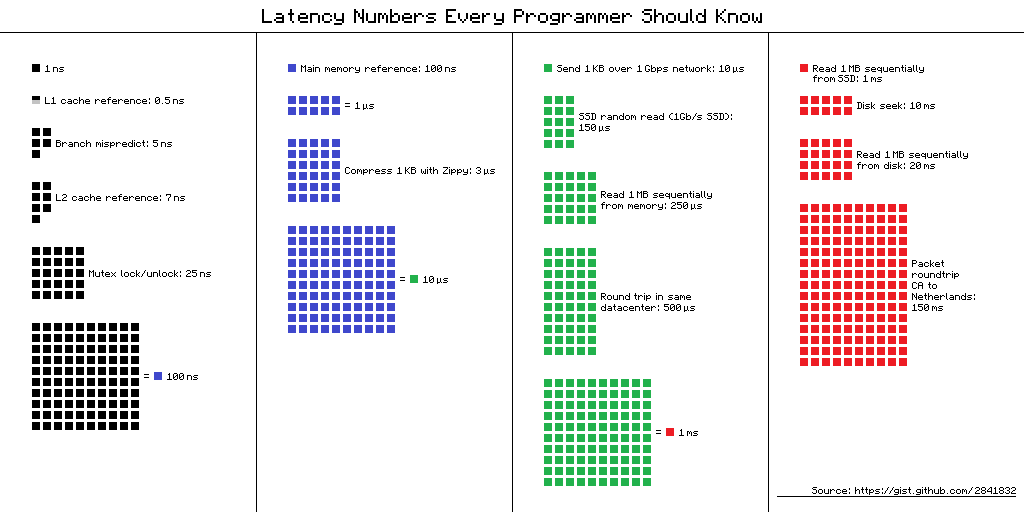
\includegraphics[width=\textwidth]{sources/appendices/images/latencies-refernece.png}
	\caption[]{Humanized visualization of the data in Table 
    \ref{tab:refernce_latencies}}.
	\label{fig:refernce_latencies}
\end{figure}

\FloatBarrier

\vspace{-2cm}
\section*{Data structures Asymptotic complexity cheatsheet}
% Please add the following required packages to your document preamble:
% \usepackage{booktabs}
% \usepackage{multirow}
% \usepackage{graphicx}
% \usepackage[table,xcdraw]{xcolor}
% If you use beamer only pass "xcolor=table" option, i.e. \documentclass[xcolor=table]{beamer}
\begin{table}[!htbp]
    \centering
    \resizebox{\textwidth}{!}{%
    \begin{tabular}{@{}lccccccccc@{}}
    \toprule
                                              & \multicolumn{8}{l}{\textbf{Time Complexities}}                                                                                                                                                                                                                                                                                                                                                  & \multicolumn{1}{l}{\textbf{Space Complexity}}             \\ \cmidrule(l){2-10} 
                                              & \multicolumn{1}{l}{\textbf{Average case}}    & \multicolumn{7}{l}{\textbf{Worst case}}                                                                                                                                                                                                                                                                                                          & \multicolumn{1}{l}{}                                      \\
    \multirow{-3}{*}{\textbf{Data Structure}} & \multicolumn{1}{l}{\textit{\textbf{Access}}} & \multicolumn{1}{l}{\textit{\textbf{Search}}} & \multicolumn{1}{l}{\textit{\textbf{Insertion}}} & \multicolumn{1}{l}{\textit{\textbf{Deletion}}} & \multicolumn{1}{l}{\textit{\textbf{Access}}} & \multicolumn{1}{l}{\textit{\textbf{Search}}} & \multicolumn{1}{l}{\textit{\textbf{Insertion}}} & \multicolumn{1}{l}{\textit{\textbf{Deletion}}} & \multicolumn{1}{l}{\multirow{-2}{*}{\textbf{Worst case}}} \\ \cmidrule(r){1-1}
    Array                                     & \cellcolor[HTML]{009901}$O(1)$               & \cellcolor[HTML]{FFC702}$O(n)$               & \cellcolor[HTML]{FFC702}$O(n)$                  & \cellcolor[HTML]{FFC702}$O(n)$                 & \cellcolor[HTML]{009901}$O(1)$               & \cellcolor[HTML]{FFC702}$O(n)$               & \cellcolor[HTML]{FFC702}$O(n)$                  & \cellcolor[HTML]{FFC702}$O(n)$                 & \cellcolor[HTML]{FFC702}$O(n)$                            \\
    Stack                                     & \cellcolor[HTML]{009901}$O(1)$               & \cellcolor[HTML]{656565}N.A.                 & \cellcolor[HTML]{009901}$O(1)$                  & \cellcolor[HTML]{009901}$O(1)$                 & \cellcolor[HTML]{009901}$O(1)$               & \cellcolor[HTML]{656565}N.A.                 & \cellcolor[HTML]{009901}$O(1)$                  & \cellcolor[HTML]{009901}$O(1)$                 & \cellcolor[HTML]{FFC702}$O(n)$                            \\
    Queue                                     & \cellcolor[HTML]{009901}$O(1)$               & \cellcolor[HTML]{656565}N.A.                 & \cellcolor[HTML]{009901}$O(1)$                  & \cellcolor[HTML]{009901}$O(1)$                 & \cellcolor[HTML]{009901}$O(1)$               & \cellcolor[HTML]{656565}N.A.                 & \cellcolor[HTML]{009901}$O(1)$                  & \cellcolor[HTML]{009901}$O(1)$                 & \cellcolor[HTML]{FFC702}$O(n)$                            \\
    Singly Linked List                        & \cellcolor[HTML]{FFC702}$O(n)$               & \cellcolor[HTML]{FFC702}$O(n)$               & \cellcolor[HTML]{009901}$O(1)$                  & \cellcolor[HTML]{FFC702}$O(n)$                 & \cellcolor[HTML]{FFC702}$O(n)$               & \cellcolor[HTML]{FFC702}$O(n)$               & \cellcolor[HTML]{009901}$O(1)$                  & \cellcolor[HTML]{FFC702}$O(n)$                 & \cellcolor[HTML]{FFC702}$O(n)$                            \\
    Doubly Linked List                        & \cellcolor[HTML]{FFC702}$O(n)$               & \cellcolor[HTML]{FFC702}$O(n)$               & \cellcolor[HTML]{009901}$O(1)$                  & \cellcolor[HTML]{009901}$O(1)$                 & \cellcolor[HTML]{FFC702}$O(n)$               & \cellcolor[HTML]{FFC702}$O(n)$               & \cellcolor[HTML]{009901}$O(1)$                  & \cellcolor[HTML]{009901}$O(1)$                 & \cellcolor[HTML]{FFC702}$O(n)$                            \\
    Hash Table                                & \cellcolor[HTML]{009901}$O(1)$               & \cellcolor[HTML]{009901}$O(1)$               & \cellcolor[HTML]{009901}$O(1)$                  & \cellcolor[HTML]{009901}$O(1)$                 & \cellcolor[HTML]{FFC702}$O(n)$               & \cellcolor[HTML]{FFC702}$O(n)$               & \cellcolor[HTML]{FFC702}$O(n)$                  & \cellcolor[HTML]{FFC702}$O(n)$                 & \cellcolor[HTML]{FFC702}$O(n)$                            \\
    Binary Search Tree                        & \cellcolor[HTML]{32CB00}$O(log_2(n))$        & \cellcolor[HTML]{32CB00}$O(log_2(n))$        & \cellcolor[HTML]{32CB00}$O(log_2(n))$           & \cellcolor[HTML]{32CB00}$O(log_2(n))$          & \cellcolor[HTML]{FFC702}$O(n)$               & \cellcolor[HTML]{FFC702}$O(n)$               & \cellcolor[HTML]{FFC702}$O(n)$                  & \cellcolor[HTML]{FFC702}$O(n)$                 & \cellcolor[HTML]{FFC702}$O(n)$                            \\
    Red-Black Tree                            & \cellcolor[HTML]{32CB00}$O(log_2(n))$        & \cellcolor[HTML]{32CB00}$O(log_2(n))$        & \cellcolor[HTML]{32CB00}$O(log_2(n))$           & \cellcolor[HTML]{32CB00}$O(log_2(n))$          & \cellcolor[HTML]{32CB00}$O(log_2(n))$        & \cellcolor[HTML]{32CB00}$O(log_2(n))$        & \cellcolor[HTML]{32CB00}$O(log_2(n))$           & \cellcolor[HTML]{32CB00}$O(log_2(n))$          & \cellcolor[HTML]{FFC702}$O(n)$                            \\
    Heap                                      & \cellcolor[HTML]{009901}$O(1)$               & \cellcolor[HTML]{656565}N.A.                 & \cellcolor[HTML]{32CB00}$O(log_2(n))$           & \cellcolor[HTML]{32CB00}$O(log_2(n))$          & \cellcolor[HTML]{009901}$O(1)$               & \cellcolor[HTML]{656565}N.A.                 & \cellcolor[HTML]{32CB00}$O(log_2(n))$           & \cellcolor[HTML]{32CB00}$O(log_2(n))$          & \cellcolor[HTML]{FFC702}$O(n)$                            \\ \bottomrule
    \end{tabular}%
    }
    \caption{Asymptotic complexities for a number of data strucutes. For time, both the average and case is reported, while for space only the worst. $O(1) < O(log_2(n)) < O(log_2(n)) < O(n) < O(nlog_2(n) < O(n^2) < O(n^3) \ldots < O(2^n) < O(n!) < O(n^n)$  }
    \label{appendix:ds_complexities}
\end{table}


\begin{figure}
    \centering
\begin{tikzpicture}
    \begin{axis}[
      grid = major,
      clip = true,
      ticks = none,
      width=0.9\textwidth,
      height=0.7\textwidth,
      every axis plot/.append style={very thick},
      axis line style = ultra thick,
      clip mode=individual,
      restrict y to domain=0:40,
      restrict x to domain=0:20,
      axis x line = left,
      axis y line = left,
      domain = 0.00:10,
      xmin = 0,
      xmax = 11,
      ymin = 0,
      ymax = 42,
      xlabel = n,
      ylabel = no. of operations,
      xlabel style = {at={(axis description cs:0.5,-0.1)},anchor=south},
      ylabel style = {at={(axis description cs:-0.08,0.5)},anchor=north},
      label style = {font=\LARGE\bf},
    ]
  \addplot [
      samples=100, 
      color=red,
  ]
  {x^2}node[above,pos=1,style={font=\Large}]{$\mathcal{O}(n^2)$};
  \addplot [
      samples=100, 
      color=blue,
  ]
  {x}node[above,pos=1,style={font=\Large}]{$\mathcal{O}(n)$};
  \addplot [
      samples=100, 
      color=orange,
  ]
  {log2 x}node[above,pos=1,style={font=\Large}]{$\mathcal{O}(\log{}n)$};
  \addplot [
      samples=100, 
      color=black,
  ]
  {x*(log2 x)}node[above,pos=1,style={font=\Large}]{$\mathcal{O}(n\log{}n)$};
  \addplot [
      samples=100, 
      color=magenta,
  ]
  {1}node[above,pos=1,style={font=\Large}]{$\mathcal{O}(1)$};
  \addplot [
      samples=100, 
      color=cyan,
  ]
  {x^(2.2)}node[above,pos=1,style={font=\Large}]{$\mathcal{O}(n^3)$};
  

  \addplot [
    samples=100,
    color=green, 
  ] gnuplot{gamma(x+3)} node[above,pos=1,style={font=\Large}]{$\mathcal{O}(n!)$};

  \addplot [
    samples=100, 
    color=yellow,
]
{2.5*2^x}node[above,pos=1,style={font=\Large}]{$\mathcal{O}(2^x)$};
  
  \end{axis}
  \end{tikzpicture}

  \caption[]{Graph showing the relative growth rates of common function used to describe algorithms.}
  \label{fig:ds_complexities:graph}
\end{figure}
%%%%%%%%%%%%%%%%%%%%%%%%%%%%%%%%%%%%%%%%%%%%
%               BIBLIOGRAPHY
%%%%%%%%%%%%%%%%%%%%%%%%%%%%%%%%%%%%%%%%%%%%

%
%from documentation
%\newacronym[⟨key-val list⟩]{⟨label ⟩}{⟨abbrv ⟩}{⟨long⟩}
%above is short version of this
% \newglossaryentry{⟨label ⟩}{type=\acronymtype,
% name={⟨abbrv ⟩},
% description={⟨long⟩},
% text={⟨abbrv ⟩},
% first={⟨long⟩ (⟨abbrv ⟩)},
% plural={⟨abbrv ⟩\glspluralsuffix},
% firstplural={⟨long⟩\glspluralsuffix\space (⟨abbrv ⟩\glspluralsuffix)},
% ⟨key-val list⟩}

\newacronym{cd}{CD}{compact disk}
\newacronym{utc}{UTC}{Coordinated Universal Time}
%\newacronym{adt}{ADT}{Atlantic Daylight Time}
%\newacronym{est}{EST}{Eastern Standard Time}
 
% Use the acronyms
\gls{utc} is 3 hours behind \gls{adt} and 10 hours ahead of \gls{est}.



%\addcontentsline{toc}{chapter}{\textcolor{ocre}{Glossary}}
%\printglossaries


%Print the glossary

\addcontentsline{toc}{chapter}{\textcolor{ocre}{Bibliography}}
%\chapter*{Bibliography}
%Print the glossary
\printbibliography	
	
%%%%%%%%%%%%%%%%%%%%%%%%%%%%%%%%%%%%%%%%%%%%
%               INDEX
%%%%%%%%%%%%%%%%%%%%%%%%%%%%%%%%%%%%%%%%%%%%	
	\cleardoublepage
	\phantomsection
	\setlength{\columnsep}{0.75cm}
	\addcontentsline{toc}{chapter}{\textcolor{ocre}{Index}}
	\printindex


	%\backmatter

\end{document}
